\documentclass[border=4pt]{standalone}
\usepackage[T1]{fontenc}
\usepackage{mathptmx}
\usepackage{amsmath,amssymb}
\usepackage{xcolor}
\usepackage{tikz}
\usetikzlibrary{positioning,arrows.meta,fit,calc,shapes.geometric,backgrounds}
\definecolor{bmain}{HTML}{0F4D92}
\definecolor{bsec}{HTML}{3775BA}
\definecolor{blight}{HTML}{DCE8F5}
\definecolor{gfill}{HTML}{DDF3DE}
\definecolor{gline}{HTML}{5BAF5B}
\definecolor{rfill}{HTML}{F6CFCB}
\definecolor{rline}{HTML}{B64342}
\definecolor{nfill}{HTML}{EFEFEF}
\definecolor{nline}{HTML}{767676}
\definecolor{ink}{HTML}{272727}
\tikzset{
  >={Stealth[length=4pt]},
  box/.style={draw=nline, fill=nfill, rounded corners=2pt, align=center, inner sep=4pt, line width=0.6pt, text=ink},
  ours/.style={draw=bmain, fill=blight, rounded corners=2pt, align=center, inner sep=4pt, line width=0.9pt, text=ink},
  data/.style={draw=gline, fill=gfill, rounded corners=2pt, align=center, inner sep=4pt, line width=0.6pt, text=ink},
  warn/.style={draw=rline, fill=rfill, rounded corners=2pt, align=center, inner sep=4pt, line width=0.6pt, text=ink},
  arr/.style={->, line width=0.8pt, draw=ink},
  lab/.style={font=\footnotesize\itshape, text=nline, align=center},
}
\newcommand{\ffpp}{FF\texttt{++}}

\begin{document}
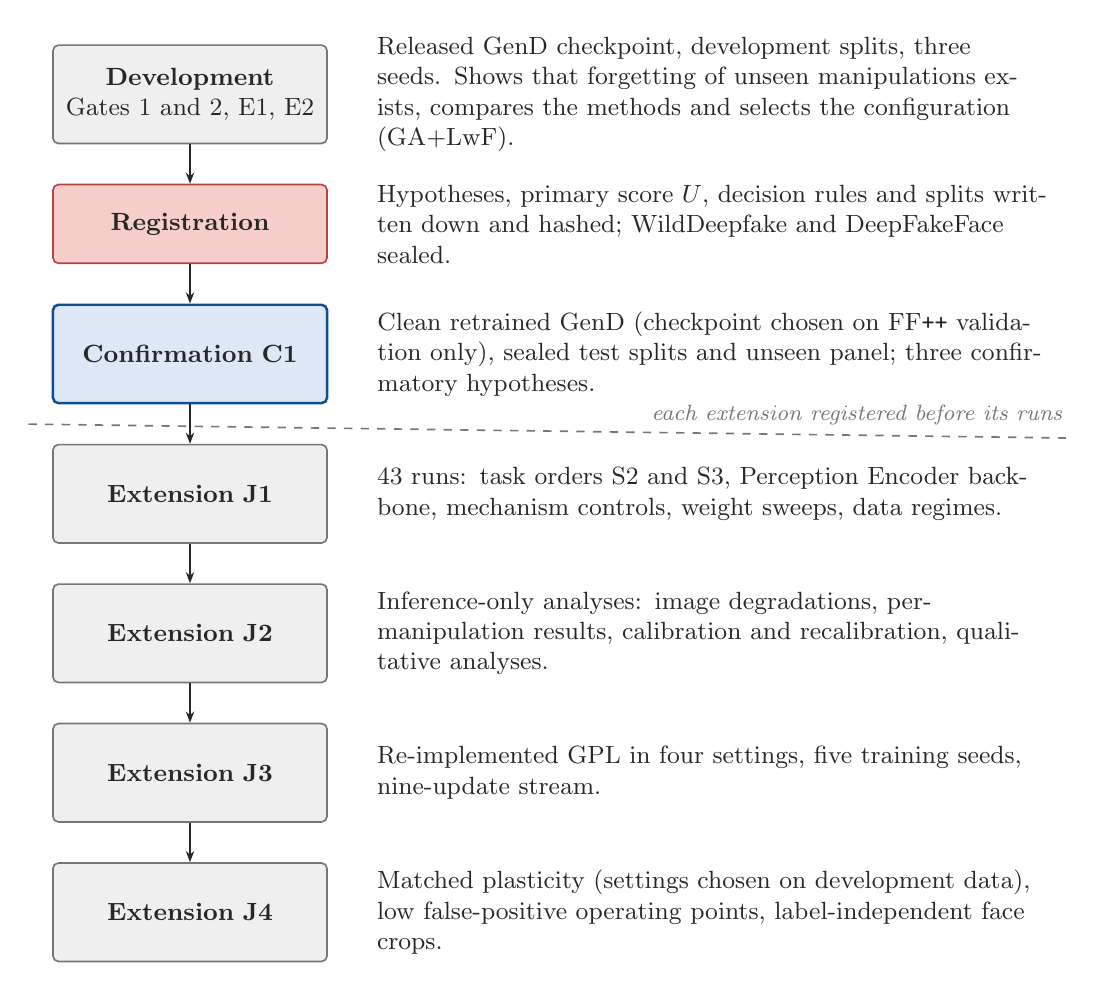
\begin{tikzpicture}[font=\small, node distance=4mm]
\tikzset{stage/.style={box, text width=3.2cm, minimum height=1.25cm}, desc/.style={align=left, text width=8.6cm, font=\small, text=ink}}
\node[box, text width=3.2cm, minimum height=1.25cm] (s1) {\textbf{Development}\\ Gates 1 and 2, E1, E2};
\node[desc, right=5mm of s1] (d1) {Released GenD checkpoint, development splits, three seeds. Shows that forgetting of unseen manipulations exists, compares the methods and selects the configuration (GA+LwF).};
\node[warn, text width=3.2cm, minimum height=1.0cm, below=5mm of s1] (s2) {\textbf{Registration}};
\node[desc, right=5mm of s2] (d2) {Hypotheses, primary score $U$, decision rules and splits written down and hashed; WildDeepfake and DeepFakeFace sealed.};
\node[ours, text width=3.2cm, minimum height=1.25cm, below=5mm of s2] (s3) {\textbf{Confirmation C1}};
\node[desc, right=5mm of s3] (d3) {Clean retrained GenD (checkpoint chosen on \ffpp{} validation only), sealed test splits and unseen panel; three confirmatory hypotheses.};
\node[box, text width=3.2cm, minimum height=1.25cm, below=5mm of s3] (s4) {\textbf{Extension J1}};
\node[desc, right=5mm of s4] (d4) {43 runs: task orders S2 and S3, Perception Encoder backbone, mechanism controls, weight sweeps, data regimes.};
\node[box, text width=3.2cm, minimum height=1.25cm, below=5mm of s4] (s5) {\textbf{Extension J2}};
\node[desc, right=5mm of s5] (d5) {Inference-only analyses: image degradations, per-manipulation results, calibration and recalibration, qualitative analyses.};
\node[box, text width=3.2cm, minimum height=1.25cm, below=5mm of s5] (s6) {\textbf{Extension J3}};
\node[desc, right=5mm of s6] (d6) {Re-implemented GPL in four settings, five training seeds, nine-update stream.};
\node[box, text width=3.2cm, minimum height=1.25cm, below=5mm of s6] (s7) {\textbf{Extension J4}};
\node[desc, right=5mm of s7] (d7) {Matched plasticity (settings chosen on development data), low false-positive operating points, label-independent face crops.};
\foreach \a/\b in {s1/s2,s2/s3,s3/s4,s4/s5,s5/s6,s6/s7} \draw[arr] (\a) -- (\b);
\draw[nline, line width=0.6pt, dashed] ($(s4.north west)+(-3mm,2.5mm)$) -- ($(d4.north east)+(1mm,2.5mm)$);
\node[lab, anchor=south east] at ($(d4.north east)+(1mm,3mm)$) {each extension registered before its runs};
\end{tikzpicture}
\end{document}
